% ######################################################################################################################

\documentclass[journal, a4paper]{IEEEtran}

\usepackage{graphicx}   % For graphics, photos, etc
\usepackage{hyperref}   % For URL and href
\usepackage{amsmath}    % For advanced mathematical formatting and symbols
\usepackage{blindtext}  % For placeholder text
\usepackage{listings}   % For code listings
\usepackage{color}      % For color

\graphicspath{{./images/}}

\definecolor{green}{rgb}{0, 0.66, 0}
\definecolor{red}{rgb}{1, 0, 0}
\definecolor{gray}{rgb}{0.5, 0.5, 0.5}
\definecolor{orange}{rgb}{1, 0.66, 0}
\definecolor{codebg}{rgb}{0.97, 0.97, 0.97}
 
\lstdefinestyle{c-style}{
  language={[ANSI]C},
  frame=single,
  backgroundcolor=\color{codebg},
  commentstyle=\itshape\color{green},
  keywordstyle=\color{blue},
  numberstyle=\tiny\color{gray},
  stringstyle=\color{orange},
  basicstyle=\fontsize{7}{7}\ttfamily,
  breakatwhitespace=false,
  breaklines=true,
  captionpos=b,
  keepspaces=true,
  numbers=left,
  numbersep=5pt,
  showspaces=false,
  showstringspaces=false,
  showtabs=false,
  tabsize=2
}

% ######################################################################################################################

\begin{document}

  \title{Neuroevolution of Augmenting Topologies}
  \author{Paul Pauls\\
          Advisor: Michael Adam}
  \markboth{Neuroevolution of Augmenting Topologies}{}
  \maketitle

\begin{abstract}
\blindtext
\end{abstract}

% ######################################################################################################################

\section{Introduction}

\IEEEPARstart{T}{his} shall be my introduction. And this shall be my citation \cite{cite01}.



% ######################################################################################################################

\section{Overview}

most commonly applied in artificial life, general game playing and evolutionary robotics.
main benefit is that Neuroevolution can be applied more widely than supervised learning algorithms [...] [as it] requires only a measure of a network's performance at a task

Neuroevolution is in competition with Gradient Descent. Around 2017 researchers at Uber stated they had found that simple structural Neuroevolution algorithms were competitive with sophisticated modern industry-standard gradient-descent deep learning algorithms, in part because Neuroevolution was found to be less likely to get stuck in local minima


\subsection{Classification of Neuroevolution Algorithms}
Conventional Neuroevolution:
evolve only the strength of the connection weights for a fixed network topology

TWEANNs (Topology and Weight Evolving Artificial Neural Network):
evolve both the topology of the network and its weights

Parallel or sequential Evolving:
A separate distinction can be made between methods that evolve the structure of ANNs in parallel to its parameters and those that develop them separately


\subsection{Genotypes and Direct/Indirect Encoding}
The question of encoding comes from the question of how do we wish to represent individuals genetically in our algorithm. The way in which we encode our individuals lays out the path for how our algorithm will handle the key evolutionary processes: selection, mutation, and crossover (also known as recombination). Any encoding will fall into one of two categories, direct or indirect.

Evolutionary algorithms operate on genotypes. In neuroevolution, a genotype is mapped to a neural network phenotype that is evaluated on some task to derive its fitness.

A direct encoding will explicitly specify everything about an individual. If it represents a neural network this means that each gene will directly be linked to some node, connection, or property of the network. This can be a binary encoding of 1s and 0s, a graph encoding (linking various nodes by weighted connections), or something even more complex. The point is that there will always be a direct connection between genotype and phenotype that is very obvious and readable. \cite{cite02}

An indirect encoding is the exact opposite. Instead of directly specifying what a structure may look like, indirect encodings tends to specify rules or parameters of processes for creating an individual. As a result, indirect encodings are much more compact. The flip side is that setting the rules for an indirect encoding can result in a heavy bias within the search space, therefore, it is much harder to create an indirect encoding without substantial knowledge about how the encoding will be used. \cite{cite02}

Phenotypes and Genomes in the context of Neuroevolution:
Let's take the example of a giraffe population that has both long-necked and short-necked giraffes. These giraffes have different phenotypes (think visible features) because they have different genomes (think codes for life).

A genotype is the genetic representation of a creature and the phenotype is the actualized physical representation of the creature. Evolutionary algorithms always heavily mirror biology, neuroevolution being no different in this respect.

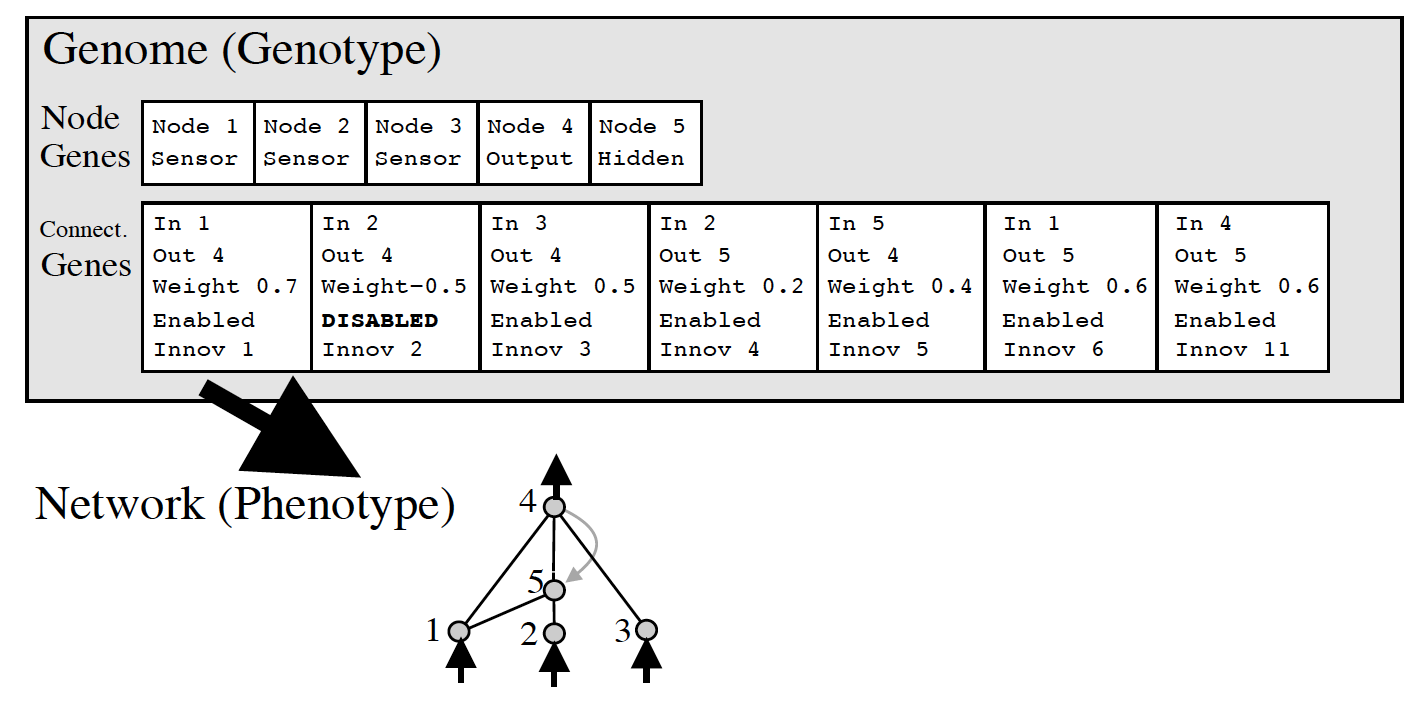
\includegraphics[width=0.45\textwidth]{Genotype_to_Phenotype_Representation}



% ######################################################################################################################

\section{NEAT}

\subsection{Mutation}
In NEAT, mutation can either mutate existing connections or can add new structure to a network. If a new connection is added between a start and end node, it is randomly assigned a weight. \cite{cite02}

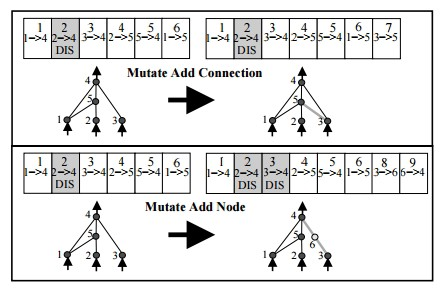
\includegraphics[width=0.45\textwidth]{Mutate_Add_Connection_and_Add_Node}


\subsection{Competing Conventions}

Another big issue with evolving the topologies of neural networks is something that the NEAT paper calls “competing conventions.” The idea is that just blindly crossing over the genomes of two neural networks could result in networks that are horribly mutated and non-functional. If two networks are dependent on central nodes that both get recombined out of the network, we have an issue. \cite{cite02}

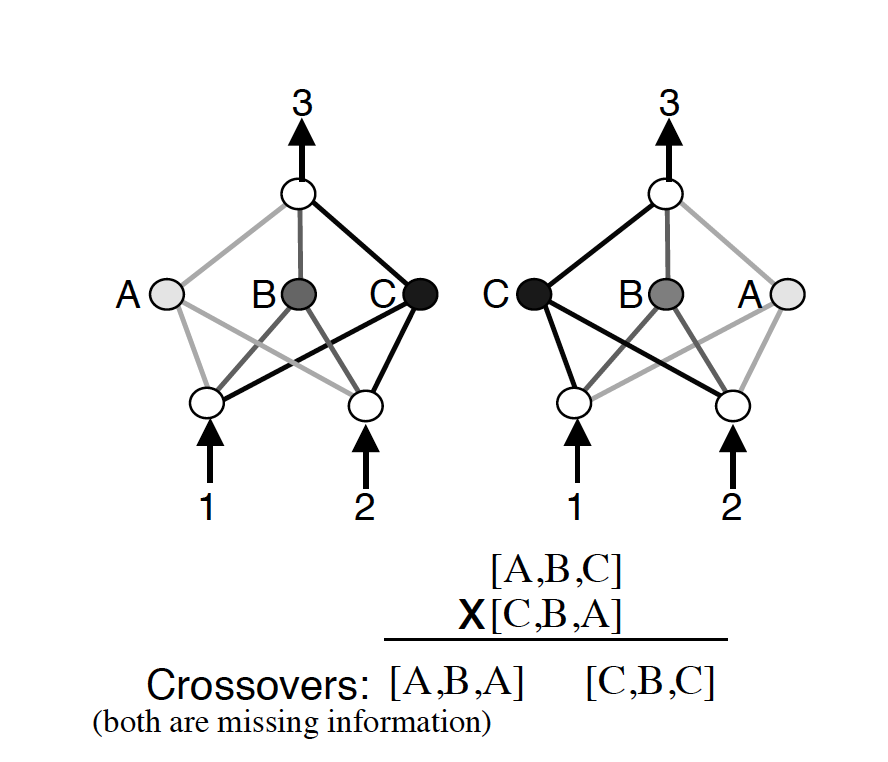
\includegraphics[width=0.45\textwidth]{Crossovers_with_Missing_Information}

More than that, genomes can be of different sizes. How do we align genomes that don’t seem to be obviously compatible? In biology, this is taken care of through an idea called homology. Homology is the alignment of chromosomes based on matching genes for a specific trait. Once that happens, crossover can happen with much less chance of error than if chromosomes were blindly mixed together. \cite{cite02}

NEAT tackles this issue through the usage of historical markings (as seen above). By marking new evolutions with a historical number, when it comes time to crossover two individuals, this can be done with much less chance of creating individuals that are non-functional. Each gene can be aligned and (potentially) crossed-over. Each time a new node or new type of connection occurs, a historical marking is assigned, allowing easy alignment when it comes to breed two of our individuals. \cite{cite02}

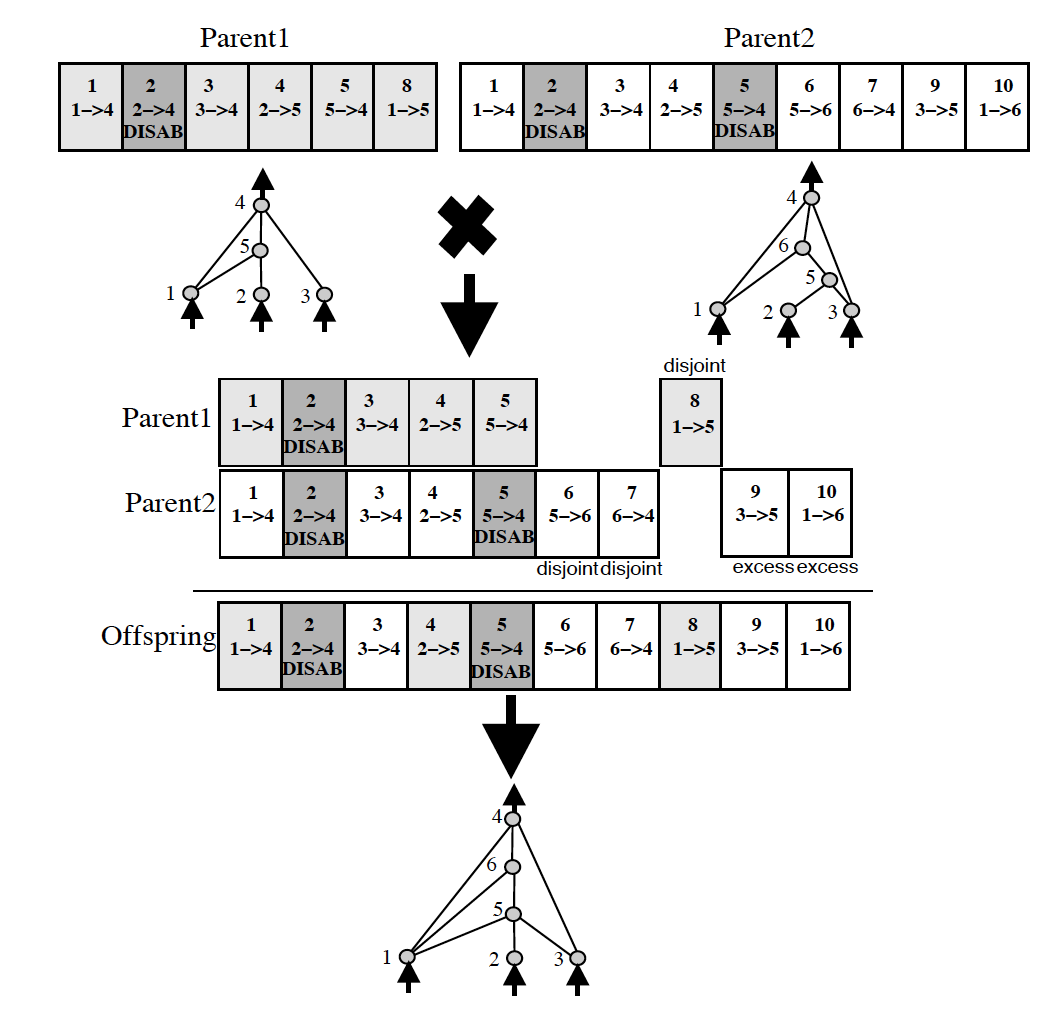
\includegraphics[width=0.45\textwidth]{Crossover_Process_Visualisation}

\subsection{Speciation}

A very interesting idea put forth in NEAT was that most new evolutions are not good ones. In fact, adding a new connection or node before any optimization of weights have occurred often leads to a lower performing individual. This puts new structures at a disadvantage. How can we protect new structures and allow them to optimize before we eliminate them from the population entirely? NEAT suggests speciation. \cite{cite02}

Speciation simply splits up the population into several species based on the similarity of topology and connections. If the competing convention problem still existed, this would be very hard to measure! However, since NEAT uses historical markings in its encoding, this becomes much easier to measure. A function for deciding how to speciate is given in the paper, but the important part to note is that individuals in a population only have to compete with other individuals within that species. This allows for new structure to be created and optimized without fear that it will be eliminated before it can be truly explored. \cite{cite02}

More than that, NEAT takes things one step forward through something called explicit fitness sharing. That means that individuals share how well they are doing across the species, boosting up higher performing species, though still allowing for other species to explore their structure optimization before being out evolved. \cite{cite02}

\subsection{Minimal Structure}

A large goal of the NEAT paper was to create a framework for evolving networks that allowed for minimal networks to be evolved. The authors did not want to create an algorithm that first found good networks and then had to reduce the number of nodes and connections after the fact. Instead, the idea was to build an algorithm that started with the minimal amount of nodes and connections, evolving complexity as time goes on if and only if it is found to be useful and necessary. \cite{cite02}

NEAT sets up their algorithm to evolve minimal networks by starting all networks with no hidden nodes. Each individual in the initial population is simply input nodes, output nodes, and a series of connection genes between them. By itself, this may not necessarily work, but when combined with the idea of speciation, this proves to be a powerful idea in evolving minimal, yet high-performing networks. \cite{cite02}



% ######################################################################################################################

\section{Conclusion}

\blindtext



% ######################################################################################################################

\begin{thebibliography}{5}

  \bibitem{cite01}
    Example Cite, {\em Source}, Apr. 2019.
    \url{www.example.com}
    
  \bibitem{cite02}
  \url{https://towardsdatascience.com/neat-an-awesome-approach-to-neuroevolution-3eca5cc7930f}

\end{thebibliography}

\end{document}
